%Time-stamp: <2013-06-18 20:31:07 amoebe>
\documentclass{article}
\usepackage{natbib}
%\usepackage{fullpage}
\usepackage{graphics}
\usepackage{amsmath}
\usepackage{amssymb}
\usepackage[utf8]{inputenc}
\usepackage{longtable} % For splitting tables over pages
\usepackage{Sweave}
\usepackage{subfig}
\usepackage{fancyhdr}
\usepackage{lastpage}
\usepackage{timestamp}
%\usepackage[section] {placeins} % http://www.douglasvanbossuyt.com/2008/11/18/la%\SweaveOpts{keep.source=TRUE} % don't remove source code comments
 % save auto-generated figures in
                                % figs/, prefixed by cant-f0creak-

\setlength{\bibsep}{0.0pt}
\setlength{\headheight}{15.2pt}
\setlength{\headsep}{12pt}
\pagestyle{fancyplain}
\fancyhf{}

\lhead{Kristine M. Yu}
\rhead{ldc-kiy plots for Example 2.2.1 in paper from 20111208, \timestamp}
\cfoot{\thepage\ of \pageref{LastPage}}

\begin{document}
  



\begin{figure}[h]
  \centering
  
\includegraphics{figs/kiy-20111208-plot-unexplained}
\caption{f0 contours from all recorded elicitation items from
    \textsc{20111208-6-kiy-ap-nps-vps}.}
  \label{fig:plot-mess}
\end{figure}

\clearpage

\begin{figure}[h]
  \centering
  
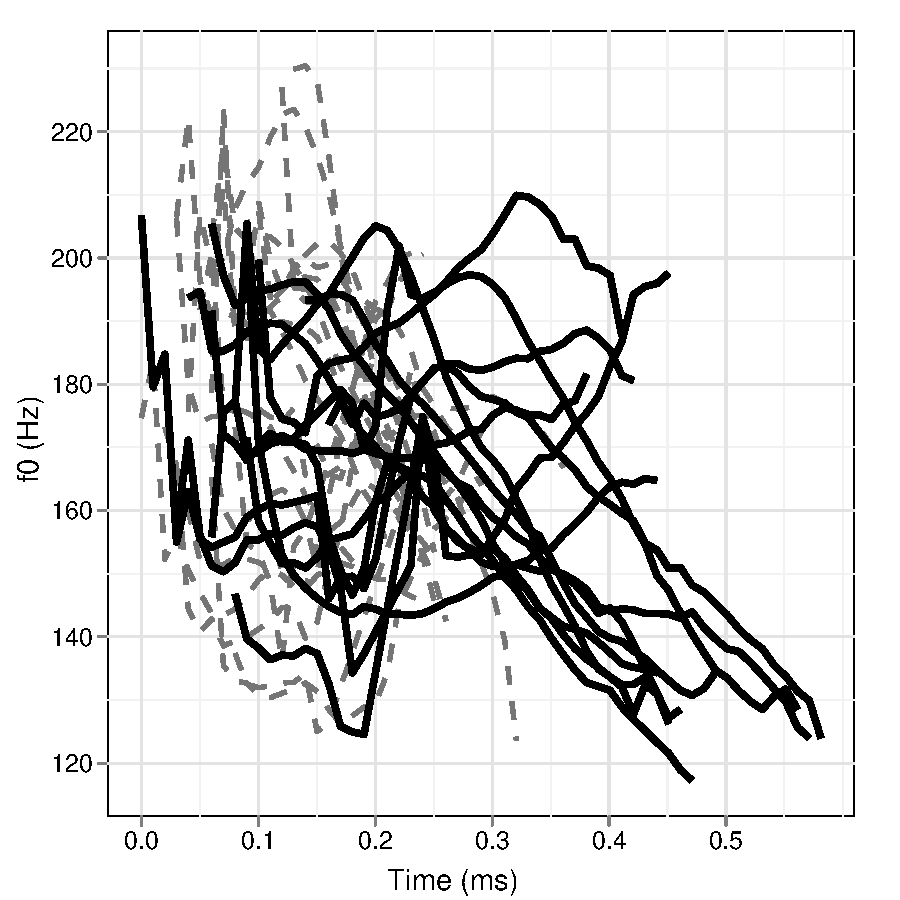
\includegraphics{figs/kiy-20111208-plot-iso}
\caption{f0 contours from all recorded elicitation items from
    \textsc{20111208-6-kiy-ap-nps-vps}.}
  \label{fig:plot-iso}
\end{figure}

\clearpage

\begin{figure}[h]
  \centering
  
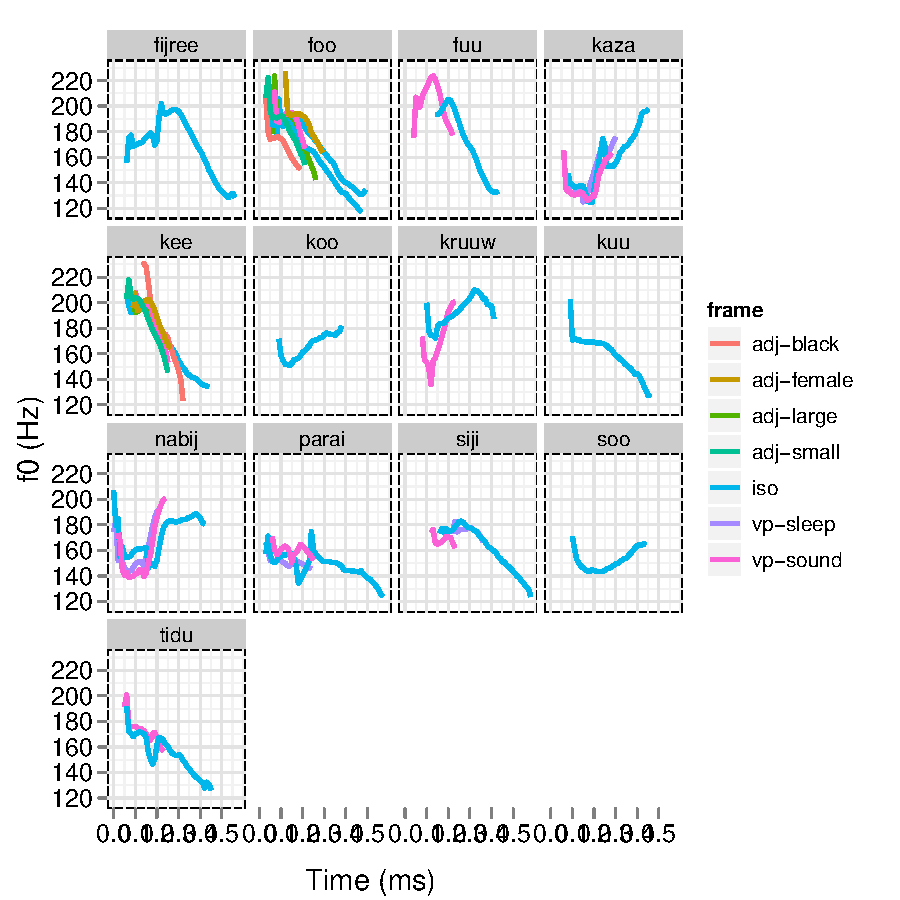
\includegraphics{figs/kiy-20111208-plot-target}
\caption{f0 contours from all recorded elicitation items from
  \textsc{20111208-6-kiy-ap-nps-vps}, faceted by target and
  color-coded within the target facets by frame. foo and kee appear
  to have the most tokens. Across frames, pitch contours for target
  words look pretty similar.}
  \label{fig:plot-target}
\end{figure}

\clearpage

Let's try looking at just foo, kee, kaza, parai, nabij, siji
\begin{figure}[h]
  \centering
  
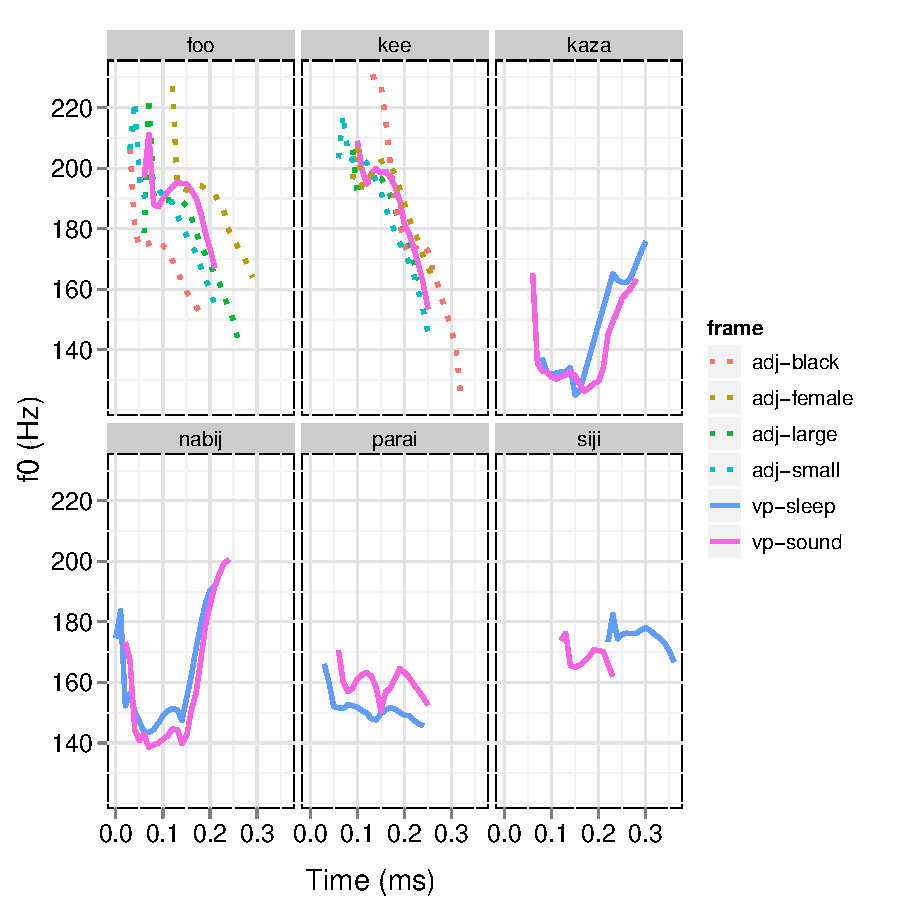
\includegraphics{figs/kiy-20111208-plot-targets-niso}

\caption{f0 contours for just foo, kaza, kee, nabij, parai, siji, no
  isolation frame. Color by frame.}
  \label{fig:plot-targets-niso}
\end{figure}

\clearpage

Compare this to if you don't do a facet plot:

\begin{figure}[h]
  \centering
  
\includegraphics{figs/kiy-20111208-plot-targets-niso-mess}

\caption{f0 contours for just foo, kaza, kee, nabij, parai, siji, no
  isolation frame. Not faceted.}
  \label{fig:plot-targets-niso-mess}
\end{figure}

\clearpage


\begin{figure}[h]
  \centering
  
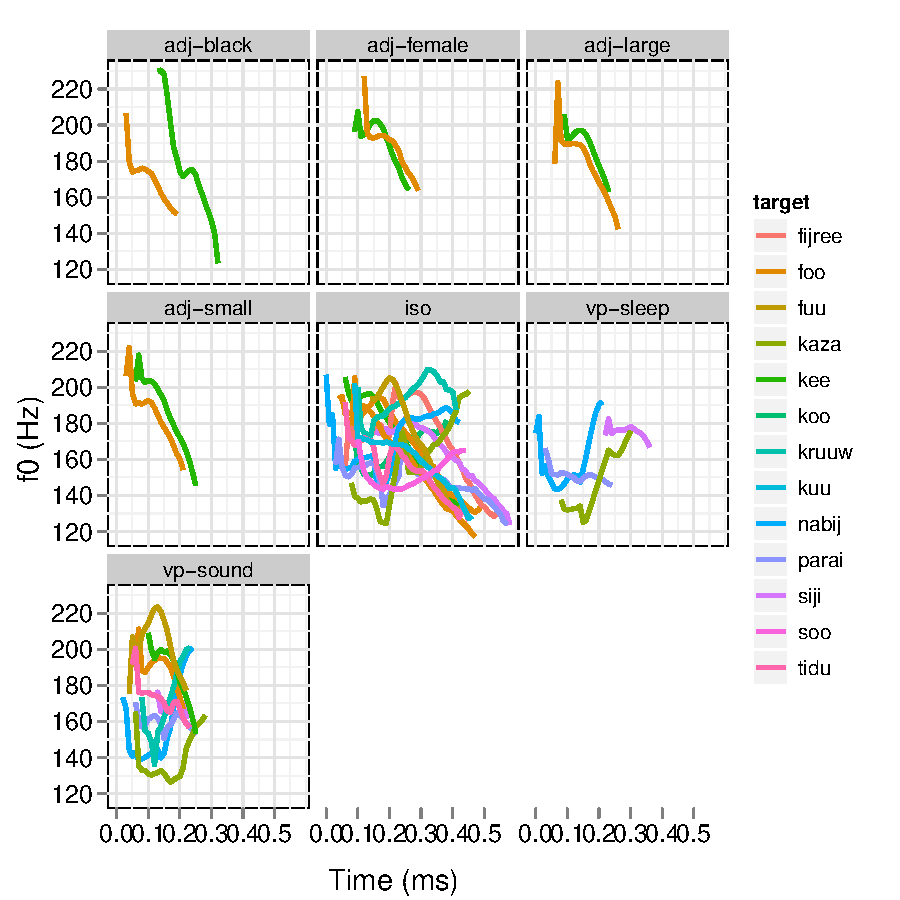
\includegraphics{figs/kiy-20111208-plot-frame}

\caption{f0 contours from all recorded elicitation items from
  \textsc{20111208-6-kiy-ap-nps-vps}, faceted by frame and
  color-coded within the target facets by target. Iso and vp-sound
  show big messes.}
  \label{fig:plot-frame}
\end{figure}

\clearpage

Let's work with only the non-adjective frames since they only have two
substitution items each.

Let's subset by syllable number and frame, lex.class.

\begin{figure}[h]
  \centering
  
\includegraphics{figs/kiy-20111208-plot-iso-syll-lex}

\caption{f0 contours from all recorded elicitation items from
  \textsc{20111208-6-kiy-ap-nps-vps} in the isolation context, color
  coded by number of syllables}
  \label{fig:plot-iso-lex}
\end{figure}

\begin{figure}[h]
  \centering
  
\includegraphics{figs/kiy-20111208-plot-niso-syll-lex}

\caption{f0 contours for vp frames, faceted by frame and color coded
  by number of syllables.}
  \label{fig:plot-niso-syll-lex}
\end{figure}


\end{document}
